\documentclass[conference]{IEEEtran}
\IEEEoverridecommandlockouts
% The preceding line is only needed to identify funding in the first footnote. If that is unneeded, please comment it out.
\usepackage{cite}
\usepackage{amsmath,amssymb,amsfonts}
\usepackage{algorithmic}
\usepackage{graphicx}
\usepackage{textcomp}
\usepackage{xcolor}
\def\BibTeX{{\rm B\kern-.05em{\sc i\kern-.025em b}\kern-.08em
    T\kern-.1667em\lower.7ex\hbox{E}\kern-.125emX}}
\begin{document}

\title{A Secure, Robust and Optimized 
Watermarking Method in Digital Images
\\
{\IEEEauthorblockN {Project Advisor: Wisam ELMASRY}}
\thanks{Identify applicable funding agency here. If none, delete this.}
}

\author{\IEEEauthorblockN{ Yaxya Mahad Wacays}
\IEEEauthorblockA{{IKU} \\
Computer Engineering\\
1800001781 \\
}
\and
\IEEEauthorblockN{Imran Makhmudov}
\IEEEauthorblockA{{IKU} \\
Computer Engineering\\
1800001143 \\
}
\and
\IEEEauthorblockN{ Muhammet Doğukan Yaraş}
\IEEEauthorblockA{{IKU} \\
Computer Engineering \\
1600001175}
}

\maketitle

\begin{abstract}
This paper aims to evaluate the practical value of utilizing DCT and DWT for watermark generation. The primary objective is to assess the effectiveness of these techniques in terms of generating watermarks that are both secure and resilient against various image processing operations and tampering attempts. A comprehensive analysis is conducted by employing different encryption methods and compression algorithms to investigate the detectability and visibility of the embedded watermarks.
\end{abstract}

\begin{IEEEkeywords}
DCT, DWT, resilient, encryption, compression
\end{IEEEkeywords}

\section{Introduction}
In the digital age, the protection of intellectual property and the prevention of unauthorized use of digital content have become increasingly critical. With the proliferation of digital media and the ease of copying and distributing information, there is a growing need for robust techniques to authenticate and protect digital assets. Watermarking has emerged as a popular method for embedding imperceptible yet identifiable information within digital media, thereby enabling the detection of unauthorized use and ensuring copyright protection. The effectiveness of a watermarking technique depends on its ability to generate watermarks that are both robust against image processing operations and imperceptible to the human visual system. 

In the realm of watermarking, the Discrete Cosine Transform and the Discrete Wavelet Transform have emerged as prominent techniques. These methods have demonstrated considerable efficacy in generating robust and invisible watermarks, effectively balancing the imperatives of invisibility and robustness. While both approaches have proven successful in watermarking applications, a comprehensive evaluation is required to fully ascertain their capabilities and identify the most suitable technique for specific scenarios. [12, 13]

By examining the detectability and resilience of the generated watermarks, we aim to provide valuable insights that will help us in selecting the most suitable transform for their specific requirements. 


\section{Related Work}

\subsection{Digital Image Watermarking Techniques: A Review}

The authors explore various methods and approaches used in the field of watermarking, with a focus on their applications and effectiveness in protecting digital images from unauthorized use and tampering. The review covers key concepts and algorithms. The authors provide an insightful analysis of the advantages and limitations of each method, emphasizing their capability to achieve a harmonious equilibrium between imperceptibility and robustness. [1]

\subsection{Fourier Image Watermarking: Print-Cam Application}
The paper aims to explore the various uses of Fourier image watermarking techniques specifically for print-cam applications. The authors propose a method that utilizes Fourier transforms for watermark embedding and extraction. Their study focuses on evaluating the robustness, visibility, and resistance against tampering of the proposed technique. This paper provides valuable insights into Fourier image watermarking in the context of print-cam applications. [8]

\subsection{A Comprehensive Survey on Digital Image Watermarking Techniques}
The authors review and analyze various methods employed in the field, including popular techniques such as spread spectrum-based watermarking, DWT, and singular value decomposition. The survey provides valuable insights into the applications, advantages, and limitations of these techniques. As a result, this resource becomes highly valuable for researchers and practitioners involved in the field of digital image watermarking. [2]


\subsection{Design and Analysis of BFO-PBFO based on totally Optimized Watermarking Algorithm for Medical Images}

A fully optimized watermarking algorithm for medical images using the BFO-PBFO optimization technique is the focus of this paper. The algorithm aims to ensure secure and robust watermarking in healthcare settings. 

The authors conduct a comprehensive analysis of the algorithm, evaluating its performance, and computational efficiency. Using this to leverage the strengths of BFO and PBFO algorithms, the proposed algorithm enhances the embedding and extraction of watermarks in medical images. [4]

This paper contributes valuable insights into the design, implementation, and analysis of the algorithm, offering significant advancements in watermarking techniques for medical images.


\subsection{Digital Watermarking Secure Scheme for Remote Sensing Image Protection}
The paper presents a secure scheme for protecting remote sensing images through digital watermarking. The proposed scheme embeds imperceptible watermarks to ensure image integrity and prevent unauthorized use. It addresses the unique challenges of remote sensing, such as high-resolution data and complex terrain. Through analysis and experimentation, the scheme's performance is evaluated in terms of watermark invisibility, robustness against attacks, and retrieval accuracy. [6]

\subsection{Robust Color Image Watermarking Scheme with High Payload Capacity using FRT-SVD}

The paper introduces a robust color image watermarking scheme with a high payload capacity using the combination of Fast Fourier Transform (FRT) and Singular Value Decomposition (SVD) techniques. The proposed scheme aims to achieve robustness against attacks while maximizing the amount of embedded information. Through extensive analysis, the scheme's performance in terms of robustness, payload capacity, and image quality is evaluated. [15]

The findings contribute to the field of color image watermarking, offering insights into an effective approach that enhances image protection while accommodating a significant payload capacity.



\section{Methodology}
The methodology employed in this project follows a systematic approach to accomplish watermark generation and embedding. The watermarking process is designed to be robust and efficient, incorporating various techniques and algorithms. The methodology consists of several key components, including:

\subsection{Discrete Cosine Transform}
The Discrete Cosine Transform (DCT) is a widely used transform technique in image processing and compression. It transforms the image from the spatial domain to the frequency domain, allowing for effective feature extraction. In this paper, the DCT technique is employed as the primary watermarking method. [2]

\subsection{Discrete Wavelet Transform}
Discrete Wavelet Transform (DWT) is a generally used technique in image processing and watermarking. It decomposes an image into different frequency sub-bands, allowing for efficient analysis and modification of image details at multiple scales. It accomplishes this by applying a series of high-pass and low-pass filters to the image, which separates the image into approximation and detail coefficients.
DWT provides a multi-resolution representation of the image, enabling the watermarking process to focus on specific frequency bands that are more suitable for embedding the watermark. The different frequency sub-bands offer varying degrees of perceptibility and robustness, allowing for a trade-off between watermark visibility and resistance to attacks. [5]

\subsection{Fast Fourier Transform}
FFT is a powerful mathematical algorithm utilized to convert images for our use case from the time or spatial domain to the frequency domain. 
It is widely employed in various applications, including image processing, audio analysis, telecommunications, and data compression. By decomposing a signal or an image into its frequency components, the FFT enables the analysis and manipulation of different frequencies present in the input. [8]
In the case of watermarking, the FFT can be used to analyze the frequency distribution of an image, identify regions of interest, and apply transformations or embedding techniques based on frequency components.

\subsection{Singular Value Decomposition}
Singular Value Decomposition (SVD) is a matrix factorization technique widely used in image processing and data analysis. It decomposes a matrix into three constituent matrices: singular values, left singular vectors, and right singular vectors. SVD provides a compact representation of the matrix by capturing its essential features and their associated directions. SVD can be used to embed watermarks by modifying the singular values or vectors. The properties of SVD, such as low-rank approximation, contribute to the robustness and capacity of the watermarking process. [19, 26]

\subsection{Compression Libraries}
Various compression libraries were considered to compress the watermark data before embedding. Our code makes use of several compression libraries, including zlib, gzip, bz2, and lzma. The code incorporates these libraries for compressing the watermark data before encryption. In our watermarking project, we primarily utilize the zlib library to compress the watermark data. Additionally, the bz2 library is employed to compress the watermark data using a different compression algorithm. However, we also tried implementing a dual compression algorithm approach, and while it was able to add additional noise to the image without any evident changes to its SSIM score, we were not able to extract the binary watermark from the final image. Therefore, for practical purposes to ensure extraction, the watermark data is compressed singularly using each respective library.



\subsection{Advanced Encryption Standard}
We incorporated the AES algorithm into our watermarking process for encrypting the binary watermark. AES is a symmetric encryption algorithm that operates on fixed-size blocks of data. Due to its exceptional level of security and efficiency, it proves to be a highly suitable choice for our specific application. AES employs complex transformations to safeguard the concealment and reliability of the data. By using AES, we ensure that the binary watermark is securely encrypted and protected against unauthorized access. [28]

\subsection{ChaCha20}
Another encryption algorithm we considered for encrypting the binary watermark is ChaCha20. ChaCha20 is a stream cipher known for its simplicity and high-speed encryption. It operates on a 512-bit state and uses a 256-bit key. 
This algorithm provides fast and efficient encryption, making it suitable for applications where performance is a crucial factor. While we did not employ ChaCha20 in our specific watermarking process, it remains a viable option for encrypting binary watermarks for comparison results. [29]

\subsection{Twofish}
We also explored the Twofish algorithm for encrypting the binary watermark. It uses a Feistel network structure, key-dependent S-boxes, and bitwise operations to ensure data confidentiality and integrity. Twofish is known for its flexibility, allowing for various key lengths and encryption modes. 
Although we did not utilize Twofish in our watermarking process, it is recognized as a strong encryption algorithm and remains a viable choice for securing binary watermarks. [30]

\subsection{Embedding Process}
The watermark embedding process involves selecting blocks from the DCT/DWT representation of the image based on their mean squared error (MSE). These selected blocks are modified by slightly adjusting their coefficients to incorporate the binary generated watermark information. This batch processing approach ensures the watermark is embedded in the blocks that it sees nets the best optimization result, balancing robustness and imperceptibility.

\subsection{Image Reconstruction/Evaluation}
The watermarked image undergoes a reconstruction step. This reconstruction involves applying the inverse DCT/DWT to the modified DCT/DWT blocks. The reconstructed image is then normalized and saved for further analysis. 
By following this methodology our project aims to achieve realistic, effective and secure binary watermark which is later embedded within the image data.


\section{Optimization}
\subsection{Particle Swarm Optimization}
To enhance the watermark embedding process, the code incorporates the PSO algorithm. PSO is an optimization system that draws inspiration from the collective behavior of a flock of birds and/or a school of fish. It effectively explores for optimal solutions in a multidimensional search space by iteratively updating the positions and velocities of particles. [33]

PSO selects the best blocks for watermark embedding by evaluating their fitness. By optimizing the selection of blocks using PSO, the code aims to maximize the embedding capacity while maintaining imperceptibility and robustness.


\subsection{Batch Processing}
Batch processing is employed in the watermark embedding process using the DCT method. By focusing on the blocks with the lowest MSE values, the generated watermark can be rooted into the regions of the test image that are less perceptually significant. [34]

\begin{figure}[htbp]
\centering
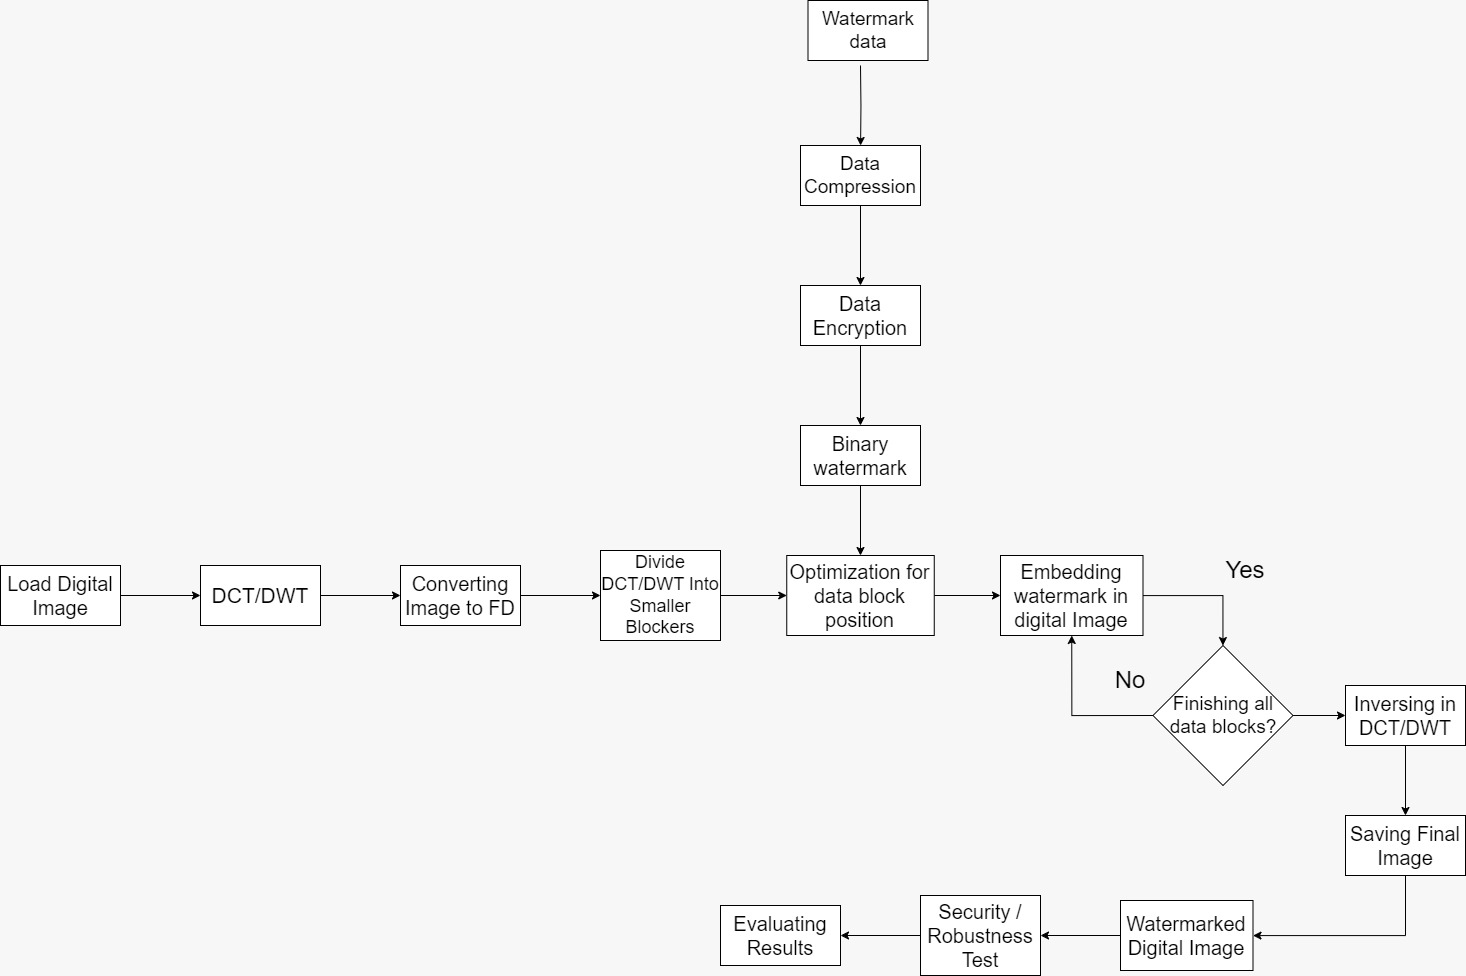
\includegraphics[width=0.9\columnwidth]{Flowchart.jpg}
\caption{Flowchart}
\label{fig}
\end{figure}
Fig. 1, shows the flowchart we utilized help us to depict the correct sequence of steps involved in our research methodology. The flowchart served as a visual roadmap, to keep us grounded and ensuring our criterias were met.
\section{Evaluation Metrics}

In order to evaluate the performance of the watermarking process, several quality assessment metrics are used. These metrics provide quantitative measures of the similarity and quality between the original image and the watermarked image. The following subsections describe the key assessment metrics employed in this project:

\subsection{Peak Signal-to-Noise Ratio (PSNR)}
Peak Signal-to-Noise Ratio quantifies the quality of the watermarked image by assessing the ratio between the maximum possible power of the signal and the power of any interfering noise. It serves as a measure of image quality, comparing the watermarked image with the original image. Higher PSNR values indicate superior image quality with reduced distortion. [35]

\begin{equation}
\text{PSNR} = 10 \cdot \log_{10} \left( \frac{{\text{MAX}^2}}{{\text{MSE}}} \right)
\tag{\ref{eq}}
\end{equation}

\subsection{Structural Similarity Index (SSIM)}
This metric takes into account factors like luminance, contrast, and structural similarity to assess the resemblance between the original and watermarked images. It provides a measure of perceived image quality, considering both global and local image features. SSIM values range from -1 to 1, with 1 indicating perfect similarity. [35]
\begin{equation}
\text{SSIM} = \frac{{(2 \mu_x \mu_y + C_1)(2 \sigma_{xy} + C_2)}}{{(\mu_x^2 + \mu_y^2 + C_1)(\sigma_x^2 + \sigma_y^2 + C_2)}}
\tag*{(2)}
\end{equation}


\subsection{Mean Square Error (MSE)}
The Mean Square Error helps us evaluate the average squared difference between the pixel values of the original and watermarked images. When the MSE values are lower, it means that the watermarked image bears a higher resemblance and exhibits better quality compared to the original image. [36]

\begin{equation}
\text{MSE} = \frac{1}{N} \sum_{i=1}^{N} (x_i - y_i)^2
\tag*{(3)}
\end{equation}


\subsection{Normalized Cross-Correlation (NCC)}
This metric allows us to measure the similarity between two images, the original and the watermarked copy, by computing the normalized dot product between them. The indicative values range from -1 to 1, with -1 illustrating the worst case where they differ too much and 1 indicating how similar it is to the original. NCC is commonly used in watermarking to assess the condition and robustness of the watermarked image. [37]

\begin{equation}
\text{NCC} = \frac{\sum_{i=1}^{N} (x_i - \bar{x})(y_i - \bar{y})}{\sqrt{\sum_{i=1}^{N} (x_i - \bar{x})^2 \sum_{i=1}^{N} (y_i - \bar{y})^2}}
\tag*{(4)}
\end{equation}


\subsection{R-test}
R-test is a statistical test used to assess the relationship between the generated watermark embedded in the image and the image itself. Similar to NCC, the R-test provides an indication of the efficacy and strength of the watermarking scheme. [38]





\section{Experimental Results}

\begin{figure}[htbp]
\centering
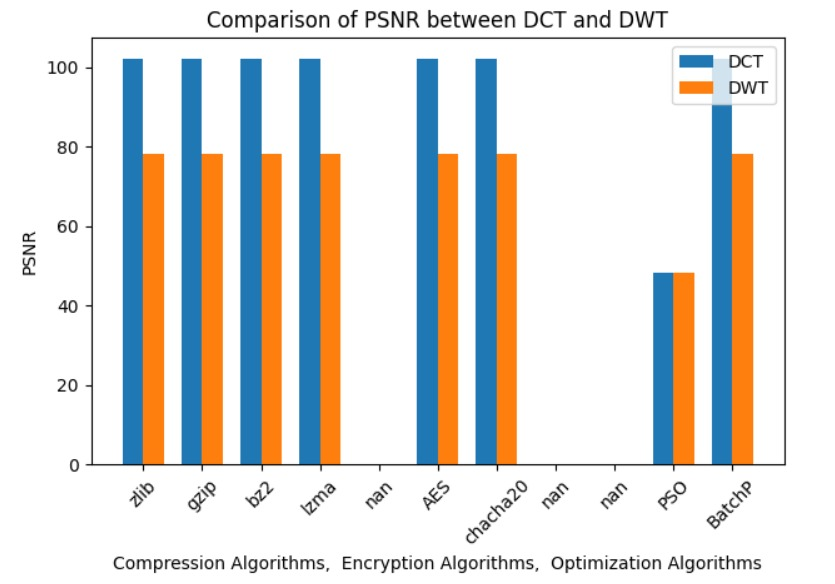
\includegraphics[width=0.9\columnwidth]{PSNR.jpg}
\caption{This figure illustrates the comparison of DCT and DWT in a specific test case scenario}
\label{fig}
\end{figure}

The results presented in Figure 2 indicate that the watermark embedding process using DCT coefficients was successful in modifying the watermarked image without causing significant visual distortion. However, the two encryption techniques employed in this test did not demonstrate clear superiority. To further investigate and provide more conclusive findings, additional tests were conducted under specific scenarios.


\begin{figure}[htbp]
\centering
\caption{DCT Test}
\label{fig}
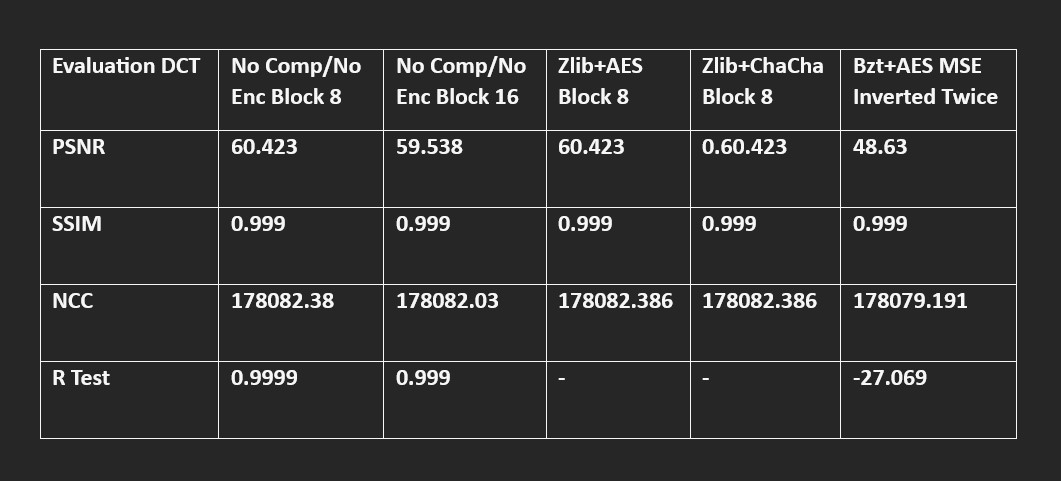
\includegraphics[width=0.9\columnwidth]{TABLE.jpg}
\end{figure}

The table presented in Figure 3 was specifically generated for additional testing purposes in order to investigate potential differences in results when utilizing DCT coefficients and embedding them into a different image file. These results shed light on the effectiveness of various techniques. To ensure a comprehensive analysis, we employed a different compression library, namely bzt, and inverted the image twice using DCT and mean square error optimization, resulting in a score of 48.63. Visually, the differences observed in the image were not significant. It is important to note that the inclusion of this table aimed to validate and verify the conclusiveness of the data collected in the previous stage.

\begin{figure}[htbp]
\centering
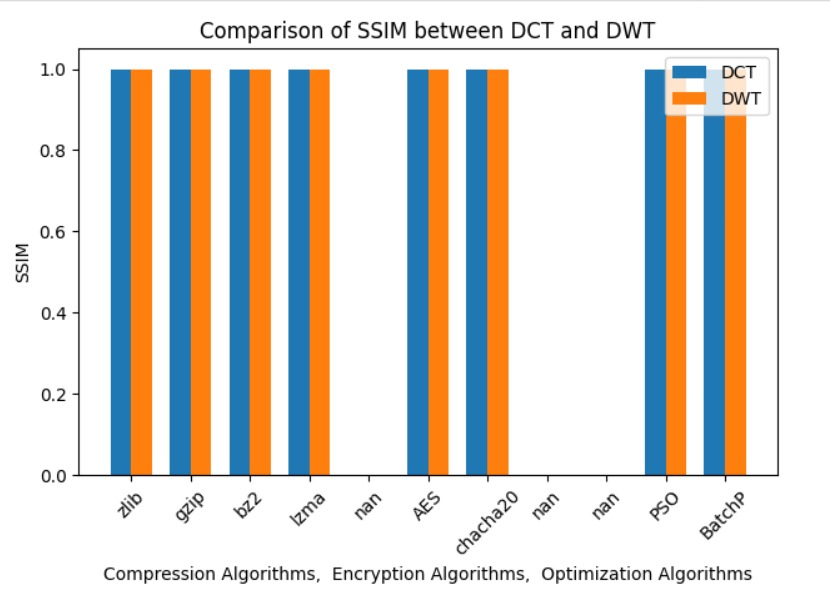
\includegraphics[width=0.9\columnwidth]{SSIM.jpg}
\caption{SSIM Comparison}
\label{fig}
\end{figure}

Regardless of the test scenario we conducted, the Structural Similarity Index remained consistent for both the DCT and the DWT methods. The SSIM values were near identical, indicating that both techniques preserved the structural information of the watermarked image in a similar manner, irrespective of the specific test conditions. This suggests that the choice between DCT and DWT may not significantly affect the SSIM performance in watermark embedding scenarios.

\begin{figure}[htbp]
\centering
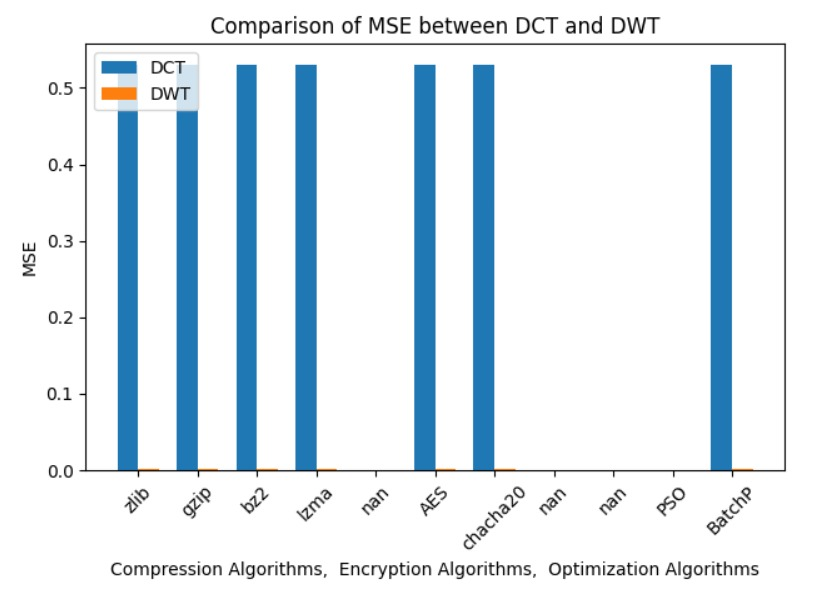
\includegraphics[width=0.9\columnwidth]{MSE.jpg}
\caption{MSE}
\label{fig}
\end{figure}

\vspace{80pt}

For the DCT method, the MSE value of 0.5307750032543858 indicates an average squared difference between the original image and the watermarked image of approximately 0.53. A lower MSE value indicates less distortion and a closer resemblance to the original image. In this case, the relatively low MSE value suggests that the watermarked image using the DCT method closely approximates the original image.

On the other hand, the DWT method yields a significantly lower MSE value of 0.0010062893081761006. This indicates a much smaller average squared difference between the original image and the watermarked image, suggesting that the watermarked image using the DWT method exhibits minimal distortion compared to the original image.


\begin{figure}[htbp]
\centering
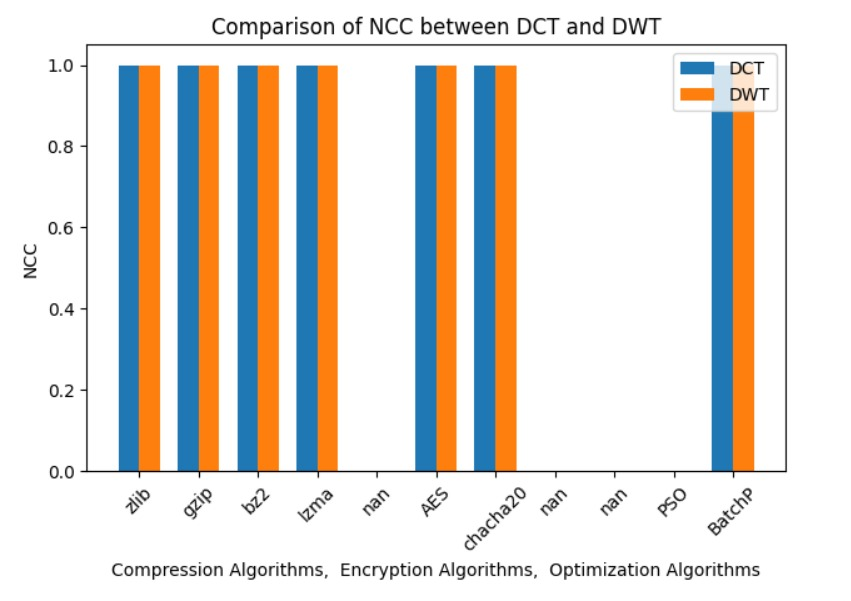
\includegraphics[width=0.9\columnwidth]{ncc.jpg}
\caption{NCC}
\label{fig}
\end{figure}

The NCC values for both methods were very close to 1, indicating a high similarity between the original and watermarked images. This clearly implies that both methods effectively preserved the integrity and quality of the original image while embedding the binary watermark.

\vspace{10pt} % Add 10pt vertical space

\section{Conclusion}

In conclusion, this study investigated the barebones effectiveness of watermark embedding techniques using DCT and DWT methods to generate invisible watermarks. The experimental results demonstrated that both methods while successful could be effectively improved by researching more efficient optimization methods.

The evaluation of performance metrics such as PSNR, SSIM, MSE, NCC, and R-test provided valuable insights into the quality and robustness of the watermarking techniques. The PSNR and SSIM scores indicated high image fidelity and similarity between the watermarked and original images for both DCT and DWT methods.

\section{Future Work}
The current watermarking model demonstrates promising results in generating invisible watermarks. However, further research can be conducted to explore optimization methods that can improve the overall performance of the model. Optimization techniques such as genetic algorithms, or deep learning-based approaches can be investigated to enhance the robustness and imperceptibility of the generated watermarks. These methods can optimize the embedding process by considering various factors such as image characteristics, watermark payload, and human visual perception.


To ensure the security and integrity of the embedded watermark, stronger encryption techniques can be employed. Advanced encryption algorithms, such as RSA (Rivest-Shamir-Adleman) [39], or ECC (Elliptic Curve Cryptography) [40], can be integrated into the watermarking process. These encryption methods can provide additional layers of protection to the watermark, making it more resistant to unauthorized removal or tampering.
In order to promote user interaction and experimentation with the watermarking model, a website can be developed with a user-friendly interface. The website can provide an API that allows users to upload images, apply watermarking techniques, and manipulate the watermark image. Users can visualize the effectiveness and robustness of the watermark by comparing the edited watermark image with the watermarked image that contains the binary watermark. 

The website can also offer additional functionality by enabling users to experiment with different algorithms for encryption, compression, optimization, and other watermarking techniques. This interactive platform will promote research, collaboration, and knowledge sharing among watermarking enthusiasts.


\begin{thebibliography}{00}
\bibitem{b1} Begum, Mahbuba, and Mohammad Shorif Uddin. “Digital Image Watermarking Techniques: A Review.” \textit{Information}, vol. 11, no. 2, MDPI, Feb. 2020, p. 110. \url{https://doi.org/10.3390/info11020110}.
\bibitem{b2} “A Comprehensive Survey on Digital Image Watermarking Techniques.” \textit{IEEE Conference Publication | IEEE Xplore}, 1 Apr. 2015, \url{ieeexplore.ieee.org/document/7279987}.
\bibitem{b3} “---.” \textit{IEEE Conference Publication | IEEE Xplore}, 1 Apr. 2015, \url{ieeexplore.ieee.org/document/7279987}.

\bibitem{b4} “Design and Analysis of BFO-PBFO Based Optimized Watermarking Algorithm for Medical Images.” \textit{IEEE Conference Publication | IEEE Xplore}, 1 Dec. 2022, \url{ieeexplore.ieee.org/document/10054270}.

\bibitem{b5} “Digital Image Watermarking Method Based on LSB and DWT Hybrid Technique.” \textit{IEEE Conference Publication | IEEE Xplore}, 23 May 2022, \url{ieeexplore.ieee.org/document/9837586}.

\bibitem{b6} “Digital Watermarking Secure Scheme for Remote Sensing Image Protection.” \textit{IEEE Journals & Magazine | IEEE Xplore}, 1 Apr. 2020, \url{ieeexplore.ieee.org/document/9089180}.

\bibitem{b7} “Digital Watermarking Techniques and Its Application Towards Digital Halal Certificate: A Survey.” \textit{IEEE Conference Publication | IEEE Xplore}, 1 Dec. 2019, \url{ieeexplore.ieee.org/document/9067988}.

\bibitem{b8} Gourrame, Khadija, et al. “Fourier Image Watermarking: Print-Cam Application.” \textit{Electronics}, vol. 11, no. 2, MDPI, Jan. 2022, p. 266. \url{https://doi.org/10.3390/electronics11020266}.

\bibitem{b9} Guo, Jia, and Miodrag Potkonjak. \textit{Watermarking Deep Neural Networks for Embedded Systems}. 2018, \url{https://doi.org/10.1145/3240765.3240862}.

\bibitem{b10} “A Hybrid Image Cryptographic and Spatial Digital Watermarking Encryption Technique for Security and Authentication of Digital Images.” \textit{IEEE Conference Publication | IEEE Xplore}, 1 Mar. 2015, \url{ieeexplore.ieee.org/document/7576563}.

\bibitem{b11} “Hybrid Multiple Watermarking Technique for Securing Medical Image Using DWT-FWHT-SVD.” \textit{IEEE Conference Publication | IEEE Xplore}, 1 May 2017, \url{ieeexplore.ieee.org/document/8075569}.

\bibitem{b12} Kumar, Mahendra. “Digital Image Watermarking Using Fractional Fourier Transform via Image Compression.” \textit{ResearchGate}, Dec. 2013, \url{https://doi.org/10.13140/RG.2.1.3010.2489}.

\bibitem{b13} Lala, Hina. \textit{Digital Image Watermarking Using Discrete Wavelet Transform}. 2017, \url{www.semanticscholar.org/paper/Digital-Image-Watermarking-using-Discrete-Wavelet-Lala/06d37fc1843e162ace2388024c0b153d4e7a524b}.

\bibitem{b14} “A Review on Digital Image Watermarking With Cryptosystem Techniques.” \textit{IEEE Conference Publication | IEEE Xplore}, 3 Apr. 2021, \url{ieeexplore.ieee.org/document/9431809}.

\bibitem{b15} “Robust Color Image Watermarking Scheme With High Payload Capacity Using FRT-SVD.” \textit{IEEE Conference Publication | IEEE Xplore}, 26 Nov. 2021, \url{ieeexplore.ieee.org/document/9702542}.

\bibitem{b16} “Robust Image Watermarking Based on Generative Adversarial Network.” \textit{IEEE Journals & Magazine | IEEE Xplore}, 1 Nov. 2020, \url{ieeexplore.ieee.org/document/9267803}.

\bibitem{b17} Sagar, Ganapathi V., et al. \textit{Convolution Based Face Recognition Using DWT and Feature Vector Compression}. 2015, \url{https://doi.org/10.1109/iciip.2015.7414814}.

\bibitem{b18} Siddeq, Mohammed M. “Using Two Levels DWT With Limited Sequential Search Algorithm for Image Compression.” \textit{Journal of Signal and Information Processing}, vol. 03, no. 01, Scientific Research Publishing, Feb. 2012, pp. 51–62. \url{https://doi.org/10.4236/jsip.2012.31008}.

\bibitem{b19} “SoRS: An Effective SVD-DWT Watermarking Algorithm With SVD on the Revised Singular Value.” \textit{IEEE Conference Publication | IEEE Xplore}, 1 June 2014, \url{ieeexplore.ieee.org/abstract/document/6933734}.
\bibitem{b20} Surekha, P., and S. Sumathi. “PERFORMANCE COMPARISON OF OPTIMIZATION TECHNIQUES ON ROBUST DIGITAL-IMAGE WATERMARKING, AGAINST ATTACKS.” \textit{Applied Artificial Intelligence}, vol. 26, no. 7, Taylor and Francis, Aug. 2012, pp. 615–44. \url{https://doi.org/10.1080/08839514.2012.687670}.
\bibitem{b21} “A Survey on Neural Trojans.” \textit{IEEE Conference Publication | IEEE Xplore}, 1 Mar. 2020, \url{ieeexplore.ieee.org/document/9137011}.
\bibitem{b22} Swathi, H. R., et al. “Image Compression Using Singular Value Decomposition.” \textit{IOP Conference Series: Materials Science and Engineering}, vol. 263, IOP Publishing, Nov. 2017, p. 042082. \url{https://doi.org/10.1088/1757-899x/263/4/042082}.
\bibitem{b23} Tao, Christopher. “Python Watermarking: OpenCV Vs PIL Vs Filestools | Towards Data Science.” \textit{Medium}, 3 Apr. 2023, \url{towardsdatascience.com/python-watermarking-old-vs-new-clunky-vs-clean-which-will-you-choose-5f4f1e75a9f3}.
\bibitem{b24} Uchida, Yusuke, et al. \textit{Embedding Watermarks Into Deep Neural Networks}. 2017, \url{https://doi.org/10.1145/3078971.3078974}.
\bibitem{b25} “Watermarking Deep Neural Networks in Image Processing.” \textit{IEEE Journals & Magazine | IEEE Xplore}, 1 May 2021, \url{ieeexplore.ieee.org/document/9093125}.
\bibitem{b26} Yildiz, Sadik, et al. “Digital Image Watermarking With Hybrid Structure of DWT, DCT, SVD Techniques and the Optimization With BFO Algorithm.” \textit{Politeknik Dergisi}, Jan. 2023, \url{https://doi.org/10.2339/politeknik.1192824}.
\bibitem{b27} Zhang, Jie. “Model Watermarking for Image Processing Networks.” \textit{arXiv.org}, 25 Feb. 2020, \url{arxiv.org/abs/2002.11088}.
\bibitem{b28} Daemen, J., \& Rijmen, V. (2002). The design of Rijndael: AES - the advanced encryption standard. Springer.
\bibitem{b29} Bernstein, D. J. (2008). ChaCha, a variant of Salsa20. Retrieved from \url{https://cr.yp.to/chacha.html}

\bibitem{b30} Schneier, B., Kelsey, J., Whiting, D., Wagner, D., Hall, C., \& Ferguson, N. (1998). The Twofish encryption algorithm: A 128-bit block cipher. Retrieved from \url{https://www.schneier.com/academic/archives/1998/09/the_twofish_encryp.html}

\bibitem{b31} Cox, I. J., Miller, M. L., Bloom, J. A., Fridrich, J., \& Kalker, T. (2002). Digital watermarking and steganography. Morgan Kaufmann.

\bibitem{b32} Kundur, D., \& Hatzinakos, D. (1999). Digital watermarking using multiresolution wavelet decomposition. Proceedings of the IEEE, 87(7), 1167-1180.


\bibitem{b33} Kennedy, J., \& Eberhart, R. (1995). Particle swarm optimization. Proceedings of IEEE International Conference on Neural Networks, 4, 1942-1948.

\bibitem{b34} Jovanov, E., O'Donnell, T., Raskovic, D., \& Cox, M. (2003). Wireless technology for data acquisition in clinical trials. Journal of Diabetes Science and Technology, 3(5), 1137-1143.

\bibitem{b35} Wang, Z., Bovik, A. C., Sheikh, H. R., \& Simoncelli, E. P. (2004). Image quality assessment: From error visibility to structural similarity. IEEE Transactions on Image Processing, 13(4), 600-612.

\bibitem{b36} Gonzalez, R. C., \& Woods, R. E. (2008). Digital Image Processing (3rd ed.). Pearson.

\bibitem{b37} Szeliski, R. (2010). Computer Vision: Algorithms and Applications. Springer.

\bibitem{b38} Cox, I. J., Miller, M. L., Bloom, J. A., Fridrich, J., \& Kalker, T. (2002). Digital watermarking and steganography. Morgan Kaufmann.

\bibitem{b39} Liu, Y., Tang, S., Liu, R., Zhang, L., & Ma, Z. (2018). Secure and robust digital image watermarking scheme using logistic and RSA encryption. Expert Systems with Applications, 97, 95-105.

\bibitem{b40} Kumar, N., Triwedi, P., & Rathore, P. S. (2017). An Adaptive Approach for image adaptive watermarking using Elliptical curve cryptography (ECC). In ICITKM (pp. 89-92).

\end{thebibliography}

\end{document}
